
\section{Supplementary material for Discussion}

\vspace*{1cm}

Using CMA-ES to explore trait values that might allow a species to survive under future climatic conditions would require several steps:
\begin{itemize}
\item define an initial state (e.g. expert parameter set)
\item identify the parameters which we allow to vary
\item define a range of values to constrain the adaptation of these parameters
\item define the initial mutation force (the step size $\sigma$), and constrain its update process (in order to avoid "unrealistic" value)
\item define the species and the study scale: for example, what it would require to maintain a beech population in some place in Southern France (e.g. Massane forest) 
\item possibly, add some perturbations during the optimization, e.g. the introduction of a new individual with a higher fitness (e.g. to mimick an assisted gene flow)
\end{itemize}

\begin{figure}[h]
\centering
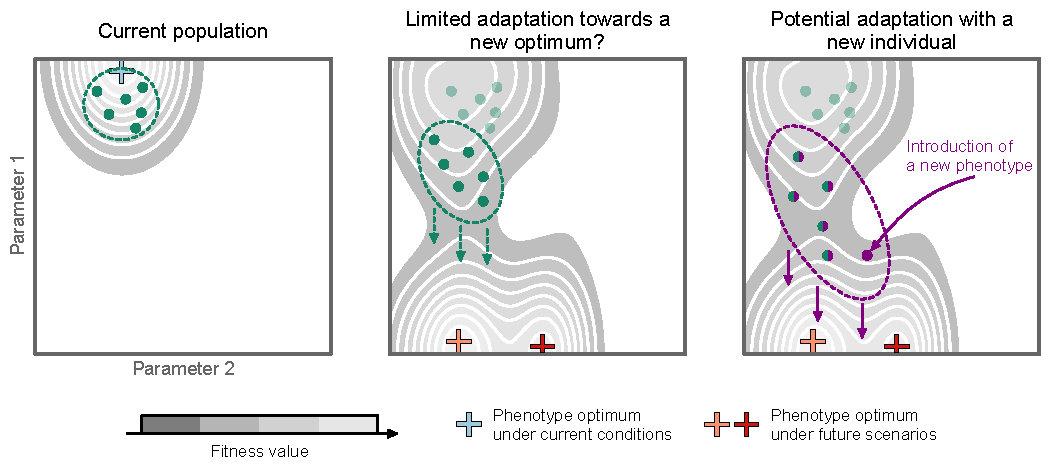
\includegraphics{discussion/figs/cmaes_evolution.pdf}
\caption{\textbf{"Bringing back CMA-ES to its evolutionary roots!"}}
\label{fig:cmaesevolution}
\end{figure}